\documentclass{article}
\usepackage[a4paper, margin=1in]{geometry}
\usepackage{graphicx} % Required for inserting images
\usepackage{hyperref}
\usepackage{cite}          % For better handling of citations
\usepackage{url}           % For handling URLs in references
\usepackage{amsmath}
\usepackage{float}
\usepackage{parskip}

\begin{document}

\begin{titlepage}
\begin{center} 

        \Huge{Report} \vspace{1cm} 
        
        \large{Pooja Yakkala} \vspace{0.3cm} 
        
    \end{center} 
\end{titlepage}

\section*{Implementation}

To build the Naïve Bayes Algorithm, I initially imported all the required libraries and downloaded the NLTK packages such as wordnet, averaged perceptron tagger, and punkt. Then I proceeded to read the dataset. Next, I pre-processed the data in the following way – First, I used fillna to fill up any empty spaces in the dataset. Then I converted the “Text” and “Label” columns to lists and cleaned that data iterating each text – lowering the text, removing punctuation from the text, removing numbers from the text and finally converting the text into tokens. To these tokens, I am applying lemmatization – meaning tagging the word with verb, noun, adverb, and adjective tags and then using lemmatizer to get the root form of that word. I have tried applying stemming but the performance of the algorithm is not that good. Lemmatization is better at this task for this dataset. But for larger datasets, it might be computationally complex. This function will return tokens of the text, labels, and vocabulary of the dataset. Then I use a feature matrix to show the number of times a word in the vocabulary is repeating in that document aka frequency of the word in that document. Here the features are equal to the number of unique words in the dataset (unigram word forms).
Then I implemented the Naïve Bayes Classifier in the following way – First, I initialized vocabulary size, class prior probabilities, the likelihood of the words, and the out-of-vocabulary constant. This Out-Of-Vocabulary (OOV) constant is used to assign a small value (1e-3) to the OOV words so that OOV words are not removed from consideration. Using different values constant resulted in different accuracies. Then, I used the fit function in which I calculated prior probabilities of each class and then used log2 for this probability. Similarly, I am calculating the likelihood probabilities of each word for each class and then using a log to stabilize the value. Finally, I use the predict class to calculate the posterior probability for each class in the document by using the prior and likelihoods computed in the fit function. As there are words in the test dataset that are not in the vocabulary or if the word has a zero probability in training, that is, if the word likelihood is -inf, I replace this value with a very small constant then it avoids zero probability and includes the outlier words as well. Finally, I use a custom confusion matrix as well as performance metrics to calculate the accuracy, precision, recall, as well as f1 score.
As for the Naïve Bayes Classifier with Laplace implementation, the way the likelihoods are calculated changes. Here smoothing applies, that is 1 is added to the word count in fit function to avoid zero probabilities. And then it calculates the score for each class based on prior and likelihood values. Following this, it selects the class with the highest score as the predicted class for the document. All the metrics are visualized with sea-born heat maps and bar graphs for comparison. For Dataset 1 (movie dataset) the accuracy is 0.60 while the accuracy for Laplace comes to 0.84. Here the low accuracy is because there are a lot of probabilities that are nearly zeros as well as OOV words were first taken to be zero and the log of such values turns out to be -inf, which causes the algorithm to misclassify (more of a random classification) leading to all the things being categorized as a single class dragging down the accuracy. When I applied the OOV constant to avoid not considering the OOV word, the accuracy was a bit better. For Dataset 2 (news reviews) the accuracy is 0.29 while Laplace comes to 0.64. I looked into why the accuracy is not good and found out that the dataset contains words that are combined into one word. To improve this accuracy, I applied the WordNinja library to split the words that are concatenated, and the accuracy increased by 0.07.


\section*{Comparison table with results on the test sets for both datasets, and with an analysis of their results (e.g., using visuals and discussion)}

\begin{figure}[H]
    \centering
    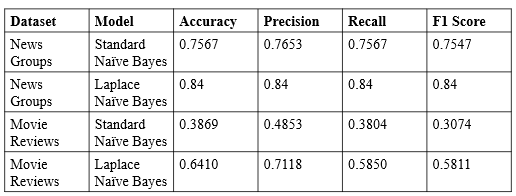
\includegraphics[width=1\textwidth]{t.png}
    \caption{Comparison Table}
    \label{fig:your_label}
\end{figure}

Upon comparing Naive Bayes with and without Laplace smoothing on the two datasets, I observed an improvement in the algorithm's performance with smoothing applied. On the Movie Review dataset, the model had only an accuracy of 75 percent, without smoothing- the biggest reasons being due to generally lower word counts, which introduced some -inf values in the log probabilities, causing a zero-probability problem. This increased the accuracy to 84 percent and gave more balanced predictions across both classes, as depicted by the confusion matrix. The improvement here is indicative of the importance of Laplace smoothing in dealing with OOV words in text classification tasks where small counts might bias or even completely alter results. 

For the Newsgroups dataset, I found a similar trend: the accuracy increased from 39 percent without smoothing to 64 percent with smoothing. One interesting observation in the smoothed results is the misclassification within the "misc" class, which often overlaps with vocabulary from the "Christian" class (most frequently) and "atheism" as well. This overlap causes a tendency to misclassify documents in "misc" as "Christian," reducing the model’s overall precision. This experience underscored the impact of smoothing on OOV handling and revealed that shared word distributions across classes, particularly in text classification, can affect accuracy in subtle but meaningful ways.

\begin{figure}[H]
    \centering
    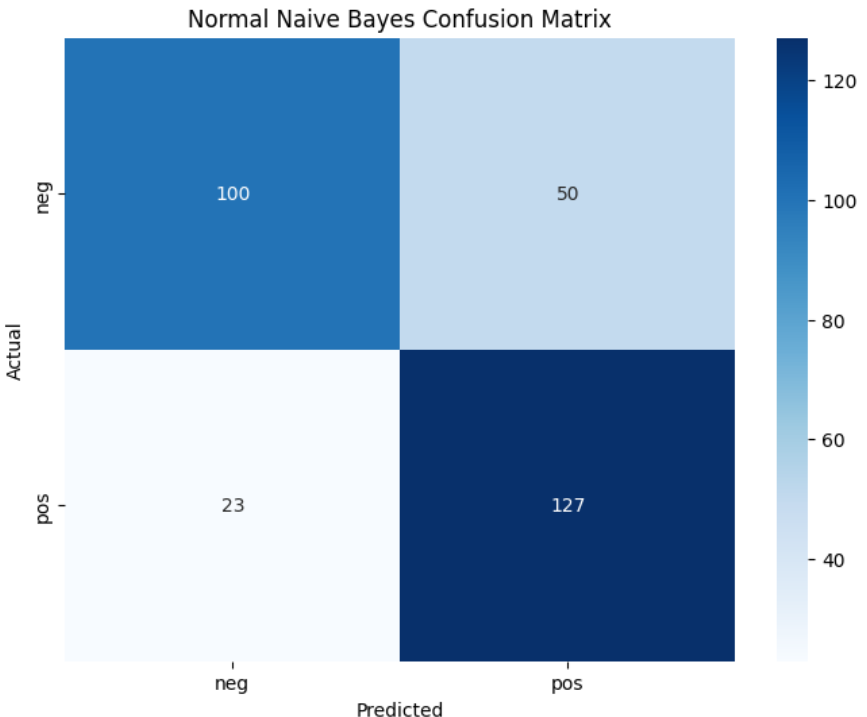
\includegraphics[width=1\textwidth]{c1.png}
    \caption{Normal Naive Bayes Confusion Matrix}
    \label{fig:your_label}
\end{figure}

\begin{figure}[H]
    \centering
    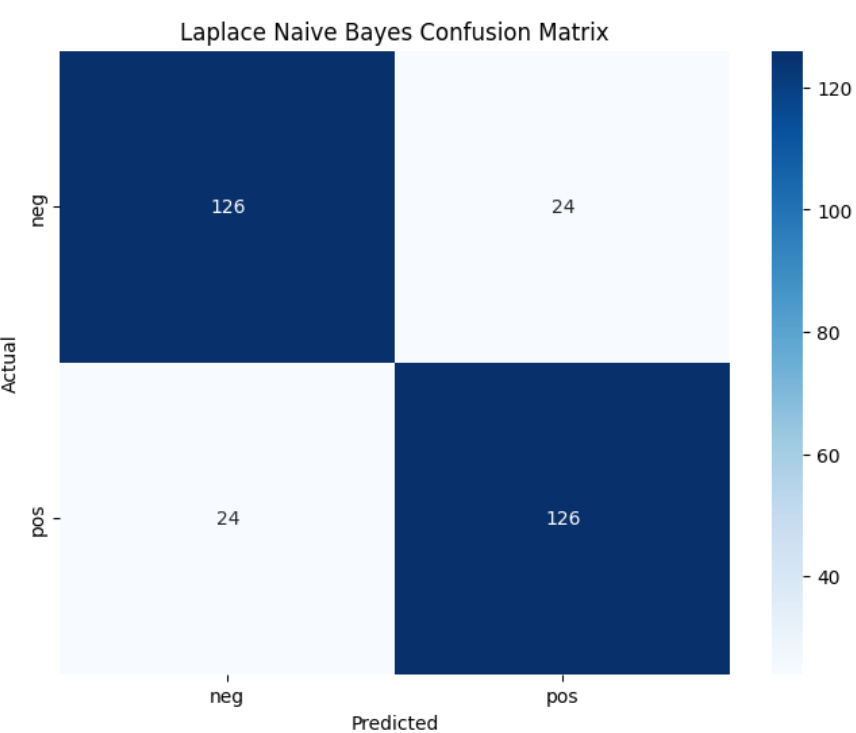
\includegraphics[width=1\textwidth]{c2.png}
    \caption{Laplace Naive Bayes Confusion Matrix}
    \label{fig:your_label}
\end{figure}

\begin{figure}[H]
    \centering
    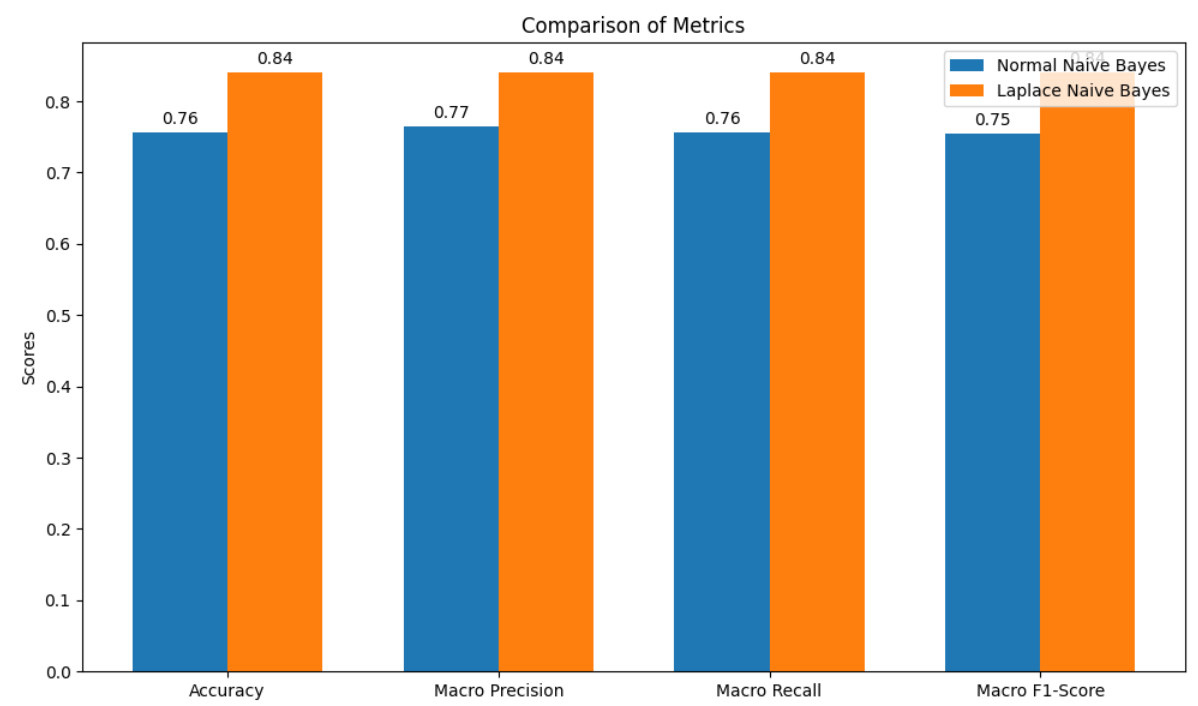
\includegraphics[width=1\textwidth]{c3.png}
    \caption{Comparison of Metrics for Movie Review Dataset}
    \label{fig:your_label}
\end{figure}

\begin{figure}[H]
    \centering
    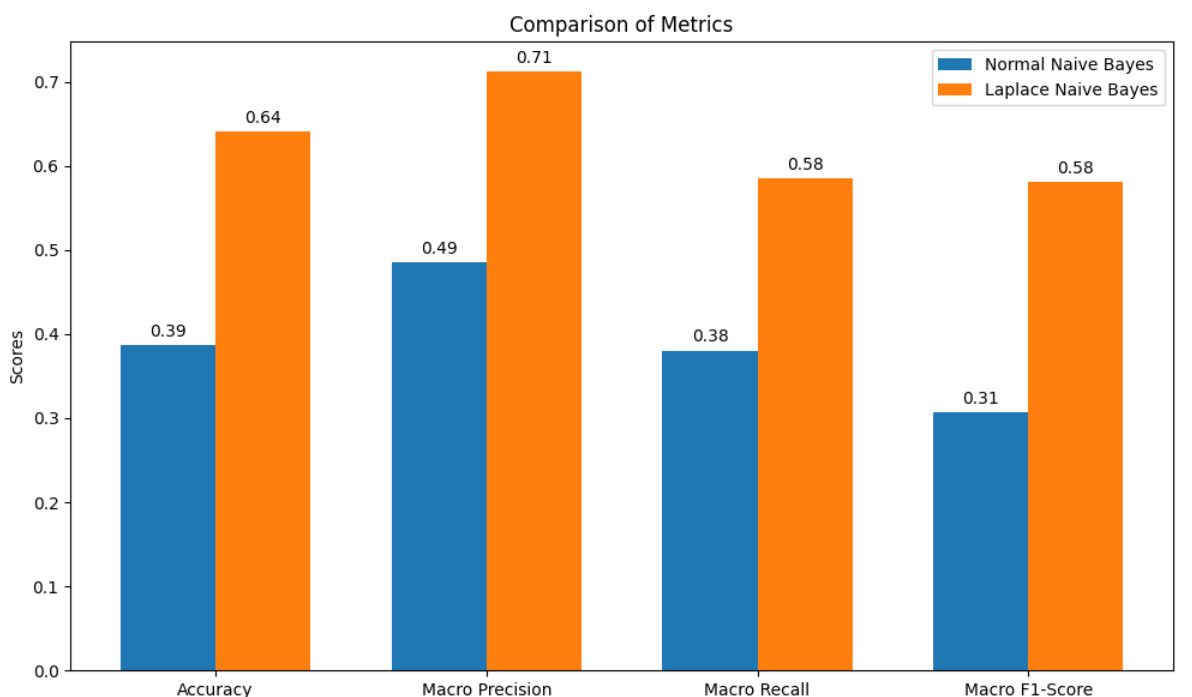
\includegraphics[width=1\textwidth]{c4.png}
    \caption{Comparison of Metrics for News Groups Dataset}
    \label{fig:your_label}
\end{figure}

\section*{Differences in the performance of Naive Bayes on both datasets.}

Naive Bayes performed extremely differently on the Movie Review and Newsgroups datasets, and this difference emanated from the nature of the data itself. The Movie Review dataset is for binary sentiment analysis, whereby the words normally have direct positive or negative sentiments. This clarity enables the model to classify the documents effectively, hence giving a high rate of accuracy. But the Newsgroups dataset is far more challenging with its multi-class classification task. Here, the accuracy is lower because of the overlapping vocabularies among categories. That means some of the words (after preprocessing the data) are present in multiple classes which makes it difficult for the model to decide on which classification is correct. 

Also, I have noticed that most of the samples are from the class 'Christian', and that gives a skewed distribution. This is another reason that causes misclassifications, especially in the "misc" class. Due to class imbalance, this algorithm will favor the Christian class since most algorithms tend to classify on the basis of the majority. This kind of behavior helps in developing the importance of having disjoint and non-intersecting vocabularies for actual classification. 

While reviewing the training data graphically, I found that since the Movie Review dataset has a balanced distribution of class labels in the Movie Review dataset it helps the algorithm perform effectively. The equal number of samples for each sentiment class creates a better training environment. On the other hand, in the newsgroup’s dataset, we have multi-class data. Here the data distribution is not equal and the Christian class has more data samples assigned to it than any other class so the simple Naive Bayes algorithm is confused. When there is an overlapping term, it classifies the data sample with the highest data samples class. This brings bias towards the Christian dataset.

\begin{figure}[H]
    \centering
    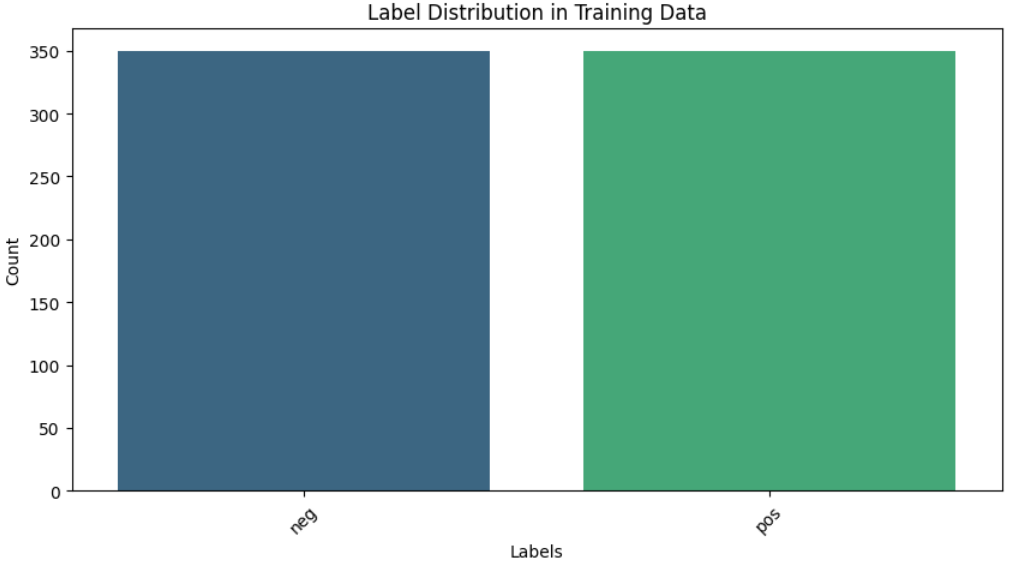
\includegraphics[width=1\textwidth]{ld1.png}
    \caption{Label Distribution in Movie Review Data}
    \label{fig:your_label}
\end{figure}

\begin{figure}[H]
    \centering
    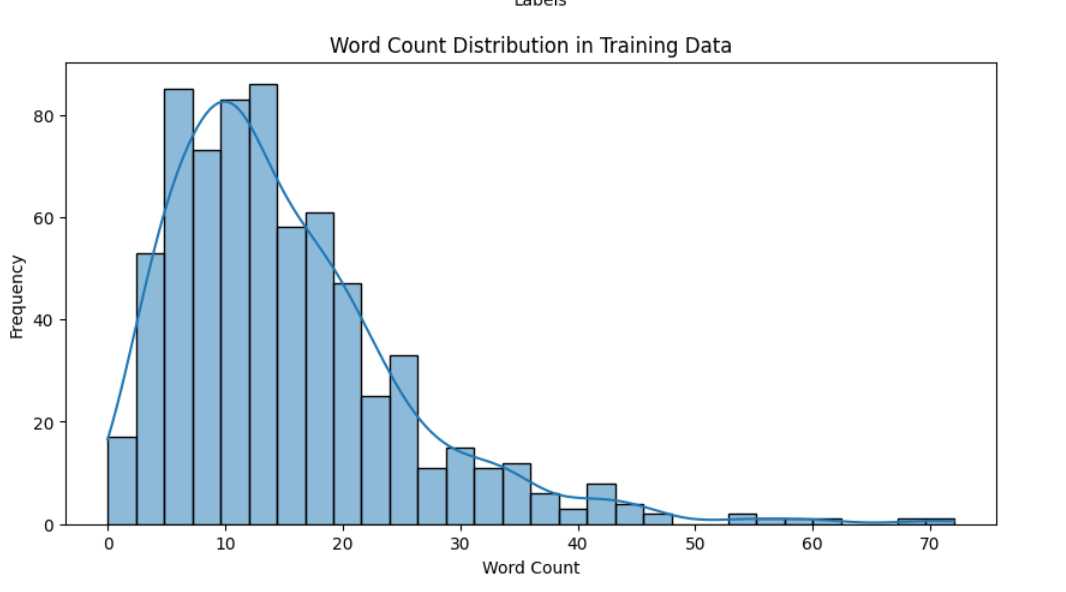
\includegraphics[width=1\textwidth]{ld2.png}
    \caption{Word Count Distribution in Movie Review Data}
    \label{fig:your_label}
\end{figure}

\begin{figure}[H]
    \centering
    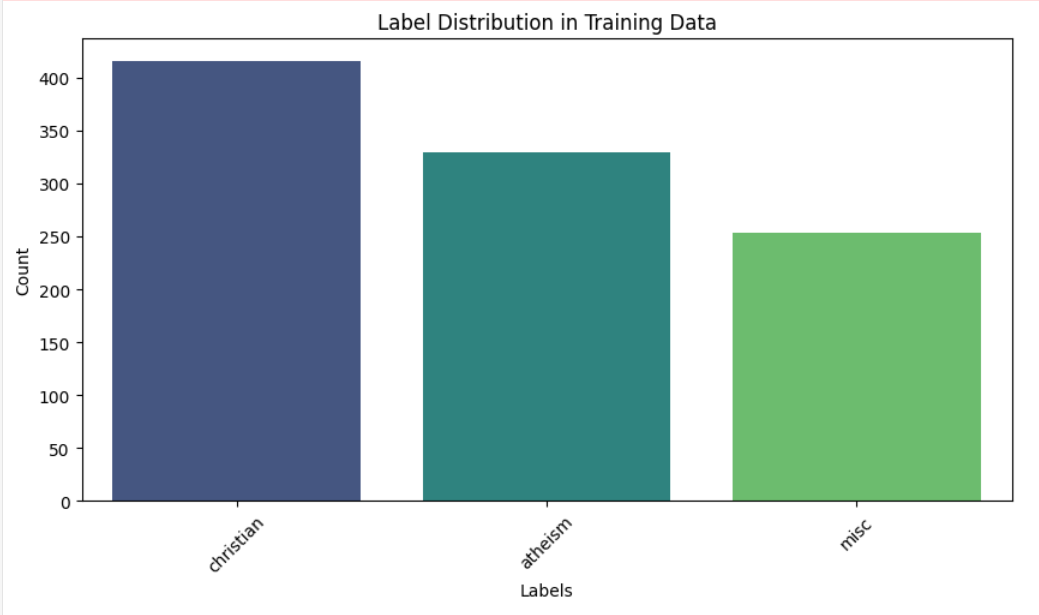
\includegraphics[width=1\textwidth]{ld3.png}
    \caption{Label Distribution in News Group Data}
    \label{fig:your_label}
\end{figure}

\begin{figure}[H]
    \centering
    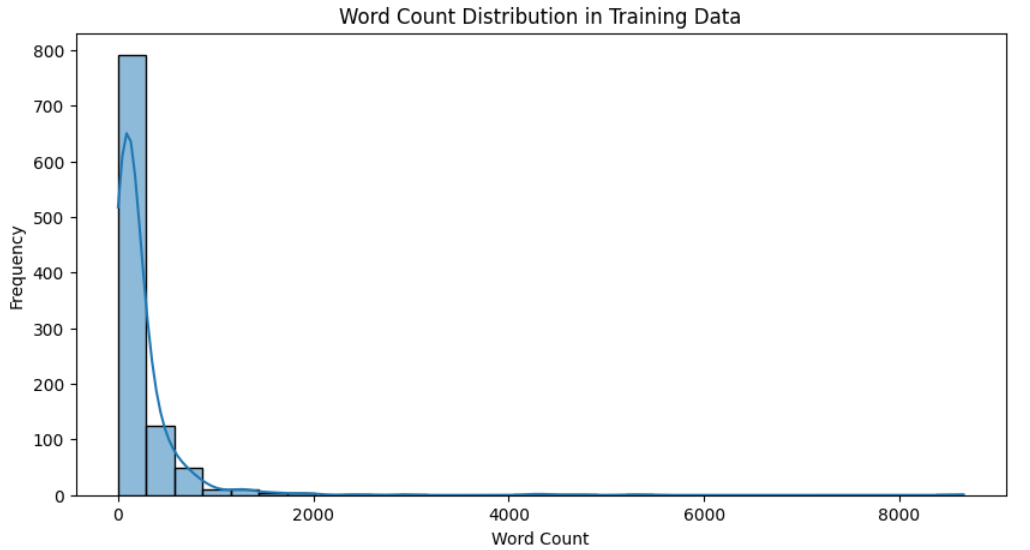
\includegraphics[width=1\textwidth]{ld4.png}
    \caption{Word Count Distribution in News Group Data}
    \label{fig:your_label}
\end{figure}

\section*{Advantages and drawbacks of the Naive Bayes algorithm.}

I noticed that the Naive Bayes algorithm has several advantages, making it attractive to try for quite a wide range of tasks on classification. First, it is strikingly simple and easy to implement. The idea that the algorithm performs is based on a relatively simple application of Bayes' theorem. Naive Bayes does extremely well on large datasets since both the training and prediction phases of this algorithm are computationally very efficient. It is particularly useful in real-time applications since predictions should be fast. Another advantage I noted is its effectiveness in dealing with high-dimensional data, such as text classification problems. The algorithm assumes the independence of features. This may also let the algorithm handle the cases where the number of features is much higher than the number of samples. This feature is particularly good for applications related to NLP, where the vocabulary size may be huge. 

However, I also came across some downsides of the Naive Bayes algorithm. One big downside is that it makes a very strong assumption of feature independence. Since many real-world features are correlated with each other, when these conditions are not met, poor performance is likely to be seen. For instance, text classification may contain some words that strongly indicate the class the text belongs to, but the algorithm does not consider this type of correlation. I also think that Naive Bayes may be problematic for imbalanced sets of data. If there are huge discrepancies in sample sizes across classes, then the algorithm starts to favor the majority class. This leads to poor classification performance for minority classes. This is especially a problem in multi-class classification, where overlapping vocabularies might confuse the algorithm and affect the precision. 

\section*{Laplace smoothing for calculating likelihood.}

My implementation of the Naive Bayes classifier with Laplace smoothing in detail. I have taken the help of two functions: fit and predict. In the fit method, after identifying the unique classes in the target labels, I initialized counts for each class and word. Then I started processing each document in the training dataset, keeping updates on the count of occurrences for a class as well as frequencies of words within the class. Having calculated the total document count, next, I estimated class prior probabilities by taking the log of the ratio of the count of documents in each class to the total document count. This modification incorporated Laplace smoothing into the likelihoods by adding one to each word count. The reason for this adjustment is to avoid a zero probability for any word that does not appear in the training data, which would skew the results. I calculated the likelihood for each class as the logarithm of the smoothed word frequency divided by the total smoothed word count, taking into account the size of the vocabulary to normalize the probabilities. I then iterated over the test documents in the predict method, computing class scores by combining class priors with the sums of the log-likelihoods of the observed words. This would allow me to obtain predictions while still maintaining the outlier words in the test set.

\section*{How expressions changed by adding Laplace smoothing in Equation 3.1}

By incorporating Laplace smoothing as in Equation 3.1, the formula for determining the likelihood of words given a class takes on a radically different form. Whereas previously it was possible, and often occurred, that the likelihood of a word given a class would be zero in the case where the word did not appear in the training data, this would result in a zero probability for any document containing that word, which for all practical purposes invalidates the entire classification process. Laplace smoothing introduces a modification that makes sure every word will have a non-zero probability even if it hadn't appeared in the training set. The modification now represents a more realistic approach toward probability estimation in text classification, with the realization that while there may be unobserved words, they indeed bear a chance of appearing in new documents. It is very important to include |V| in the denominator, which is the size of the vocabulary. This change normalizes the likelihoods across all possible words; otherwise, probabilities would skew into a small class of frequently occurring words. Adding the |V| to the denominator balances out the probabilities, allowing me to capture a better representation of the probability of each word to appear in each class. This ultimately led to the better performance of the text classification in given datasets.


\section*{Hugin-Lite}

After launching Hugin-Lite, I placed the nodes for "Cloudy," "Sprinkler," "Rain," and "Wet Grass" into the network structure shown in Figure 1, making sure the links among them were correctly connected with respect to their dependency. Then, I defined the CPTs for each node: the probabilities of "Sprinkler" and "Rain" given "Cloudy" and the probabilities of "Wet Grass" given "Sprinkler" and "Rain." After I compiled the network just to test for any errors in my building, I ran a simulation by setting the evidence variable "Wet Grass" to true to find out what the probability became of the "Sprinkler" being on and of its raining. I compared these results against my previous calculations to assess the stability and accuracy of Bayesian network predictions. The results obtained both through hand calculation and through the use of a software are the same, amounting to 70.48 or 0.7048 for rain and 42.78 for a sprinkler; this therefore sums up that it is raining.

\begin{figure}[H]
    \centering
    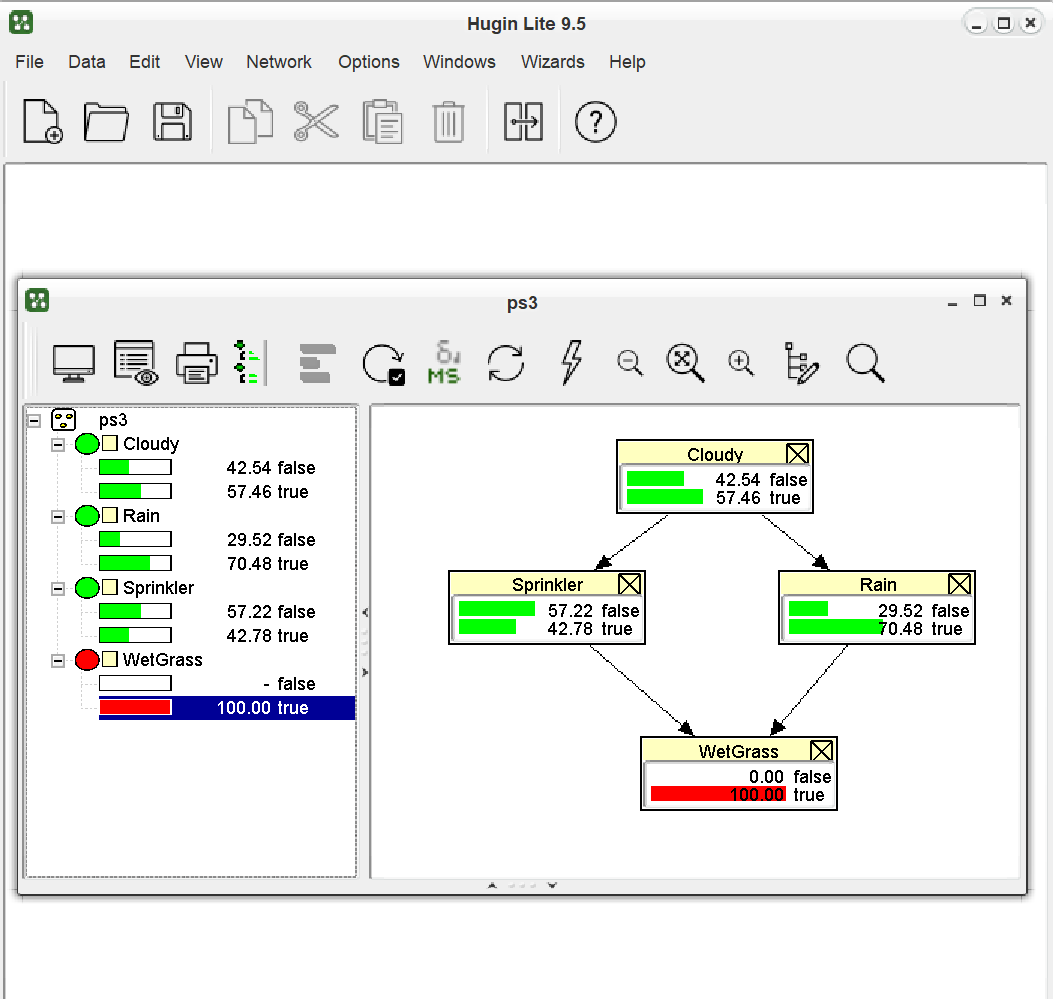
\includegraphics[width=1\textwidth]{hugin.png}
    \caption{Hugin Tree}
    \label{fig:your_label}
\end{figure}

\section*{Conditional independence as it relates to the above Bayes Network.}

In the frame of a Bayesian network, conditional independence means that some variables can be taken as independent, given knowledge of the state of a third variable. For instance, I found that the nodes "Sprinkler" and "Rain" are conditionally independent given the node "Cloudy." The fact that I learned whether it was cloudy or not does not provide new information on either Raining or Sprinkler State being On. Also, I observed that the node "Wet Grass" is dependent on both "Sprinkler" and "Rain." Once I know the states of those two nodes, though, the probability of the grass being wet is independent of the "Cloudy" node. It is this characteristic of conditional independence that allows the algorithm to break up an otherwise intractable computation of joint probabilities into smaller pieces. Coupling with the described relationships allows me to model complex probabilistic scenarios in an effective manner, with clarity about the relationships of the variables.

\end{document}


